\documentclass{article}
\usepackage[utf8]{inputenc}
\usepackage{amsmath}
\usepackage{amssymb}
\usepackage{mathtools}
\usepackage{paralist}
\usepackage{tikz}
\usepackage{enumerate}
\usepackage[margin=1.3in]{geometry}
\usepackage[english]{babel}
\usepackage{graphicx}
\usepackage{subfig}
\usepackage{mathrsfs}
\usepackage[nottoc]{tocbibind}
\usepackage{parskip} % For space between paragraphs instead of first-line indents
\usepackage{verbatim}
\usepackage[linesnumbered,ruled]{algorithm2e}
\usepackage[toc,page]{appendix}

\newtheorem{theorem}{Theorem}[section]
\newtheorem{lemma}[theorem]{Lemma}
\newtheorem{proposition}[theorem]{Proposition}
\newtheorem{corollary}[theorem]{Corollary}

\newenvironment{proof}[1][Proof]{\begin{trivlist}
\item[\hskip \labelsep {\bfseries #1}]}{\end{trivlist}}
\newenvironment{definition}[1][Definition]{\begin{trivlist}
\item[\hskip \labelsep {\bfseries #1}]}{\end{trivlist}}
\newenvironment{example}[1][Example]{\begin{trivlist}
\item[\hskip \labelsep {\bfseries #1}]}{\end{trivlist}}
\newenvironment{remark}[1][Remark]{\begin{trivlist}
\item[\hskip \labelsep {\bfseries #1}]}{\end{trivlist}}

\newcommand{\qed}{\nobreak \ifvmode \relax \else
      \ifdim\lastskip<1.5em \hskip-\lastskip
      \hskip1.5em plus0em minus0.5em \fi \nobreak
      \vrule height0.75em width0.5em depth0.25em\fi}
      
\DeclareMathOperator*{\argmin}{arg\,min}
\SetKwComment{Comment}{$\triangleright$\ }{}


\title{PowerGridsReport2}
\author{Eric Lee }
\date{August 2016}

\begin{document}
\section{Overiew}
We are given a linear differential algebraic equation (DAE)
\begin{equation} \label{DAELinear}
Ez' = \mathcal{J} z
\end{equation}
Then the solution to (\ref{DAELinear}) has the form
\begin{equation}\label{DAESolution}
z(t) = \sum_{i = 1}^{k} c_i e^{\mu_it}v_i = \sum_{i = 1}^{k} e^{\mu_it}d_i
\end{equation}
Where $\langle \mu_i,v_i \rangle$ are the non-infinite \textit{eigenpairs} of the generalized eigenvalue problem $\mathcal{J} v_i = \mu_i Ev_i $, the $v_i$ are restricted to have unit length, and $c_i$ are some constants determined by the initial condition. We can fold in our constants into our eigenvectors i.e. rewrite our solution into a slightly more compact form with $d_i = c_i v_i$. 

If one has a set of sensors, known as Phasor Measurement Units or PMUs, placed around the power system outputting a signal $f(t)$, then $f(t)$ can be explained mathematically as 
\begin{equation}\label{PMUSolution}
f(t) = Hz(t) = \sum_{i = 1}^{k} e^{\mu_it}Hd_i
\end{equation}
Note that $H$ simply picks out a subset of $z(t)$, since voltage readings are in the set of algebraic variables. So to be more precise, we get the partial eigenpairs 
$\langle \mu_i,Hv_i \rangle$ from the sensors


\section{Back to the Beginning}
Given a dictionary of contingency matrices
$$ \mathcal{D} =  \{ J_1, J_2, \dots, J_n \} $$
And a set of sensor readings 
$$ \mathcal{P} =  \{ \langle \lambda_1,x_1 \rangle, \langle \lambda_1,x_2 \rangle, \dots, \langle \lambda_n,x_n \rangle \} $$
We want to state some notion of ``distance'' $\mathcal{D} \times \mathcal{P} \rightarrow \mathbb{R}$ 
\subsection{$M(\lambda, x, J)$}
We previously defined this notion of distance as
\begin{equation}
M(\lambda, x, J) = \min_{\alpha, y} \bigg{ \| } \bigg{(}E {\lambda} - J\bigg{)}
\begin{pmatrix}
\alpha x \\
y
\end{pmatrix}
     \bigg{ \| }_2^2
\end{equation}
$$ \text{subject to } \alpha^2 + \|y\|_2^2 = 1$$
 With 
$\langle \lambda,x \rangle \in \mathcal{P}$ and $J \in \mathcal{D}$.
However, this not the most robust method. Let's say that $$\bar{\alpha}, \bar{y} = \argmin_{\alpha,y} M(\lambda, x, J)$$ i.e. $\bar{\alpha}$ and $\bar{y}$ are solutions to the non-noisy problem. 
 Then we can find a simple upper bound by plugging $\bar{\alpha}$ and $\bar{y}$ into the noisy optimization problem
\begin{equation}
M(\lambda + \delta, x + \epsilon, J) = \min_{\alpha, y} \bigg{ \| } \bigg{(}E (\lambda + \delta) - J\bigg{)}
\begin{pmatrix}
\alpha (x + \epsilon) \\
y
\end{pmatrix}
     \bigg{ \| }_2^2
\end{equation}
$$ \text{subject to } \alpha^2 + \|y\|_2^2 = 1$$


$$\leq 
M(\lambda, x, J) + 
\bigg{\|} \delta E \begin{pmatrix}
\bar{\alpha} (x + \epsilon) \\
\bar{y}
\end{pmatrix} + (E {\lambda} - J )
\begin{pmatrix}
\bar{\alpha} \epsilon \\
0
\end{pmatrix}
\bigg{\|}_2^2
$$

$$ \leq M(\lambda, x, J) + \epsilon\lambda_{max}(E {\lambda} - J)$$ 
where $\lambda_{max}(A)$ is the largest eigenvector in absolute value of $A$. Note that this is not necessarily the ideal upper bound; the $\lambda_{max}$ term gives us some problems. This upper bound is (somewhat) achieved in experimental data, as we will see in a bit



\subsection{$L(\lambda, x, J)$}
Perhaps there is no need to fit the rest of the eigenvector. Let's examine a simpler measure of ``distance'':
\begin{equation}L(\lambda, x, J) = \min_y \|Hy - x\|_2^2 \end{equation}
$$\text{subject to } y \in \Lambda(J - \lambda E)$$
Where $\Lambda(A)$ is the smallest invariant subspace of $A$ i.e. the eigenvectors corresponding to eigenvalues in some spectral interval $[-\delta, \delta]$. This is equivalent to the optimization problem
$$L(\lambda, x, J) = \min_z \|Sz - x\|_2^2$$
$$ S = H*\Lambda(J - \lambda E)$$
Which we solve by first calculating $S$ and then solving a very small least-squares problem. How does $L(\lambda + \delta, x + \epsilon, J)$ perform? Assume once again that 
$$\bar{z} = \argmin _z\|Sz - x\|_2^2$$
Then noting that $S$ does not change by definition, our error will simply be 
$$\|S\bar{z} - x - \epsilon\|_2^2 \leq L(\lambda, x, J) + \epsilon $$
Note that the amount of error incurred is $\mathcal{O}(\epsilon)$ instead of $\mathcal{O}(\epsilon \lambda_{max})$, which is an upgrade. This is reflected in some simple experimental results

\begin{figure}
\centering
\textbf{A Simple Comparison of $L(\lambda,x,J)$ and $M(\lambda,x,J)$}
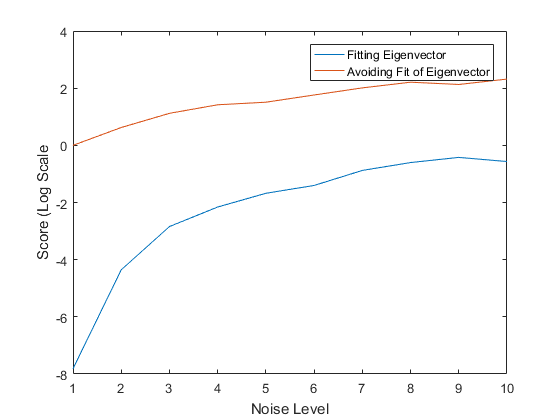
\includegraphics[width=13cm]{Comparison1.png}
\caption{Fitting Error of both $L(\lambda,x,J)$ and $M(\lambda,x,J)$ calculated by setting J to be a random matrix of size 200 and E to be the identity. We took H to be the sensing matrix $[e_1, e_2, ... e_{10}]$ where $e_i$ is the i-th unit vector, and added noise to the partial eigenpairs obtained from H. The scaling is logarithmic and indeed, $L(\lambda,x,J)$ and $M(\lambda,x,j)$ are roughly three orders of magnitude apart, which makes sense as the maximal eigenvalue of $J - \lambda E$ was roughly 95. Note that the upper bound on $M$ is roughly achieved because in our expriments, the angles between the fitted and true $y$ (the rest of the eigenvector not seen by the sensor) was very small. }
\end{figure}

\section{Getting Muddled Between Contingencies}
We want small errors in our notion of distance in the hopes that relativedistances will be roughly preserved given some noise in our sensor readings $\mathcal{P}$. Let us first consider $M(\lambda, x, J)$  

To be more precise about this problem, let's say that the correct contingency (without loss of generality) is $J$ and the incorrect contingencies are $J + U_i$ for some matrix $U_i$. Recall that the previous upper bounds in the noisy case is
$$ M(\lambda + \delta, x + \epsilon, J) \leq M(\lambda, x, J) + \epsilon\lambda_{max}(E {\lambda} - J)$$ 
Let us now consider

\begin{equation}
M(\lambda + \delta, x + \epsilon, J + U_i) = \min_{\alpha, y} \bigg{ \| } \bigg{(}E (\lambda + \delta) - J - U_i\bigg{)}
\begin{pmatrix}
\alpha (x + \epsilon) \\
y
\end{pmatrix}
     \bigg{ \| }_2^2
\end{equation}
$$ \text{subject to } \alpha^2 + \|y\|_2^2 = 1$$

$$ \leq M(\lambda , x, J) + \epsilon\lambda_{max}(E {\lambda} - J) + \bigg{\|}U_i
\begin{pmatrix}
\alpha (x + \epsilon) \\
y
\end{pmatrix}\bigg{\|}_2^2
$$ 
However, if $\|U_i\|$ is not large enough in comparison $\lambda_{max}$, we may not be able to identify distinguish contingencies properly. It is worth noting that indeed, this bound isn't necessarily the tightest, but this fact is supported once again by experimental evidence.

Analysis of $L(\lambda, x, J)$ is a bit harder. In particular, I am not sure how to characterize the perturbation of the smallest eigenvector to the matrix $\lambda E - J + U_i$. 
\begin{figure}
\centering
\textbf{A Comparison of $L(\lambda,x,J)$ and $M(\lambda,x,J)$}
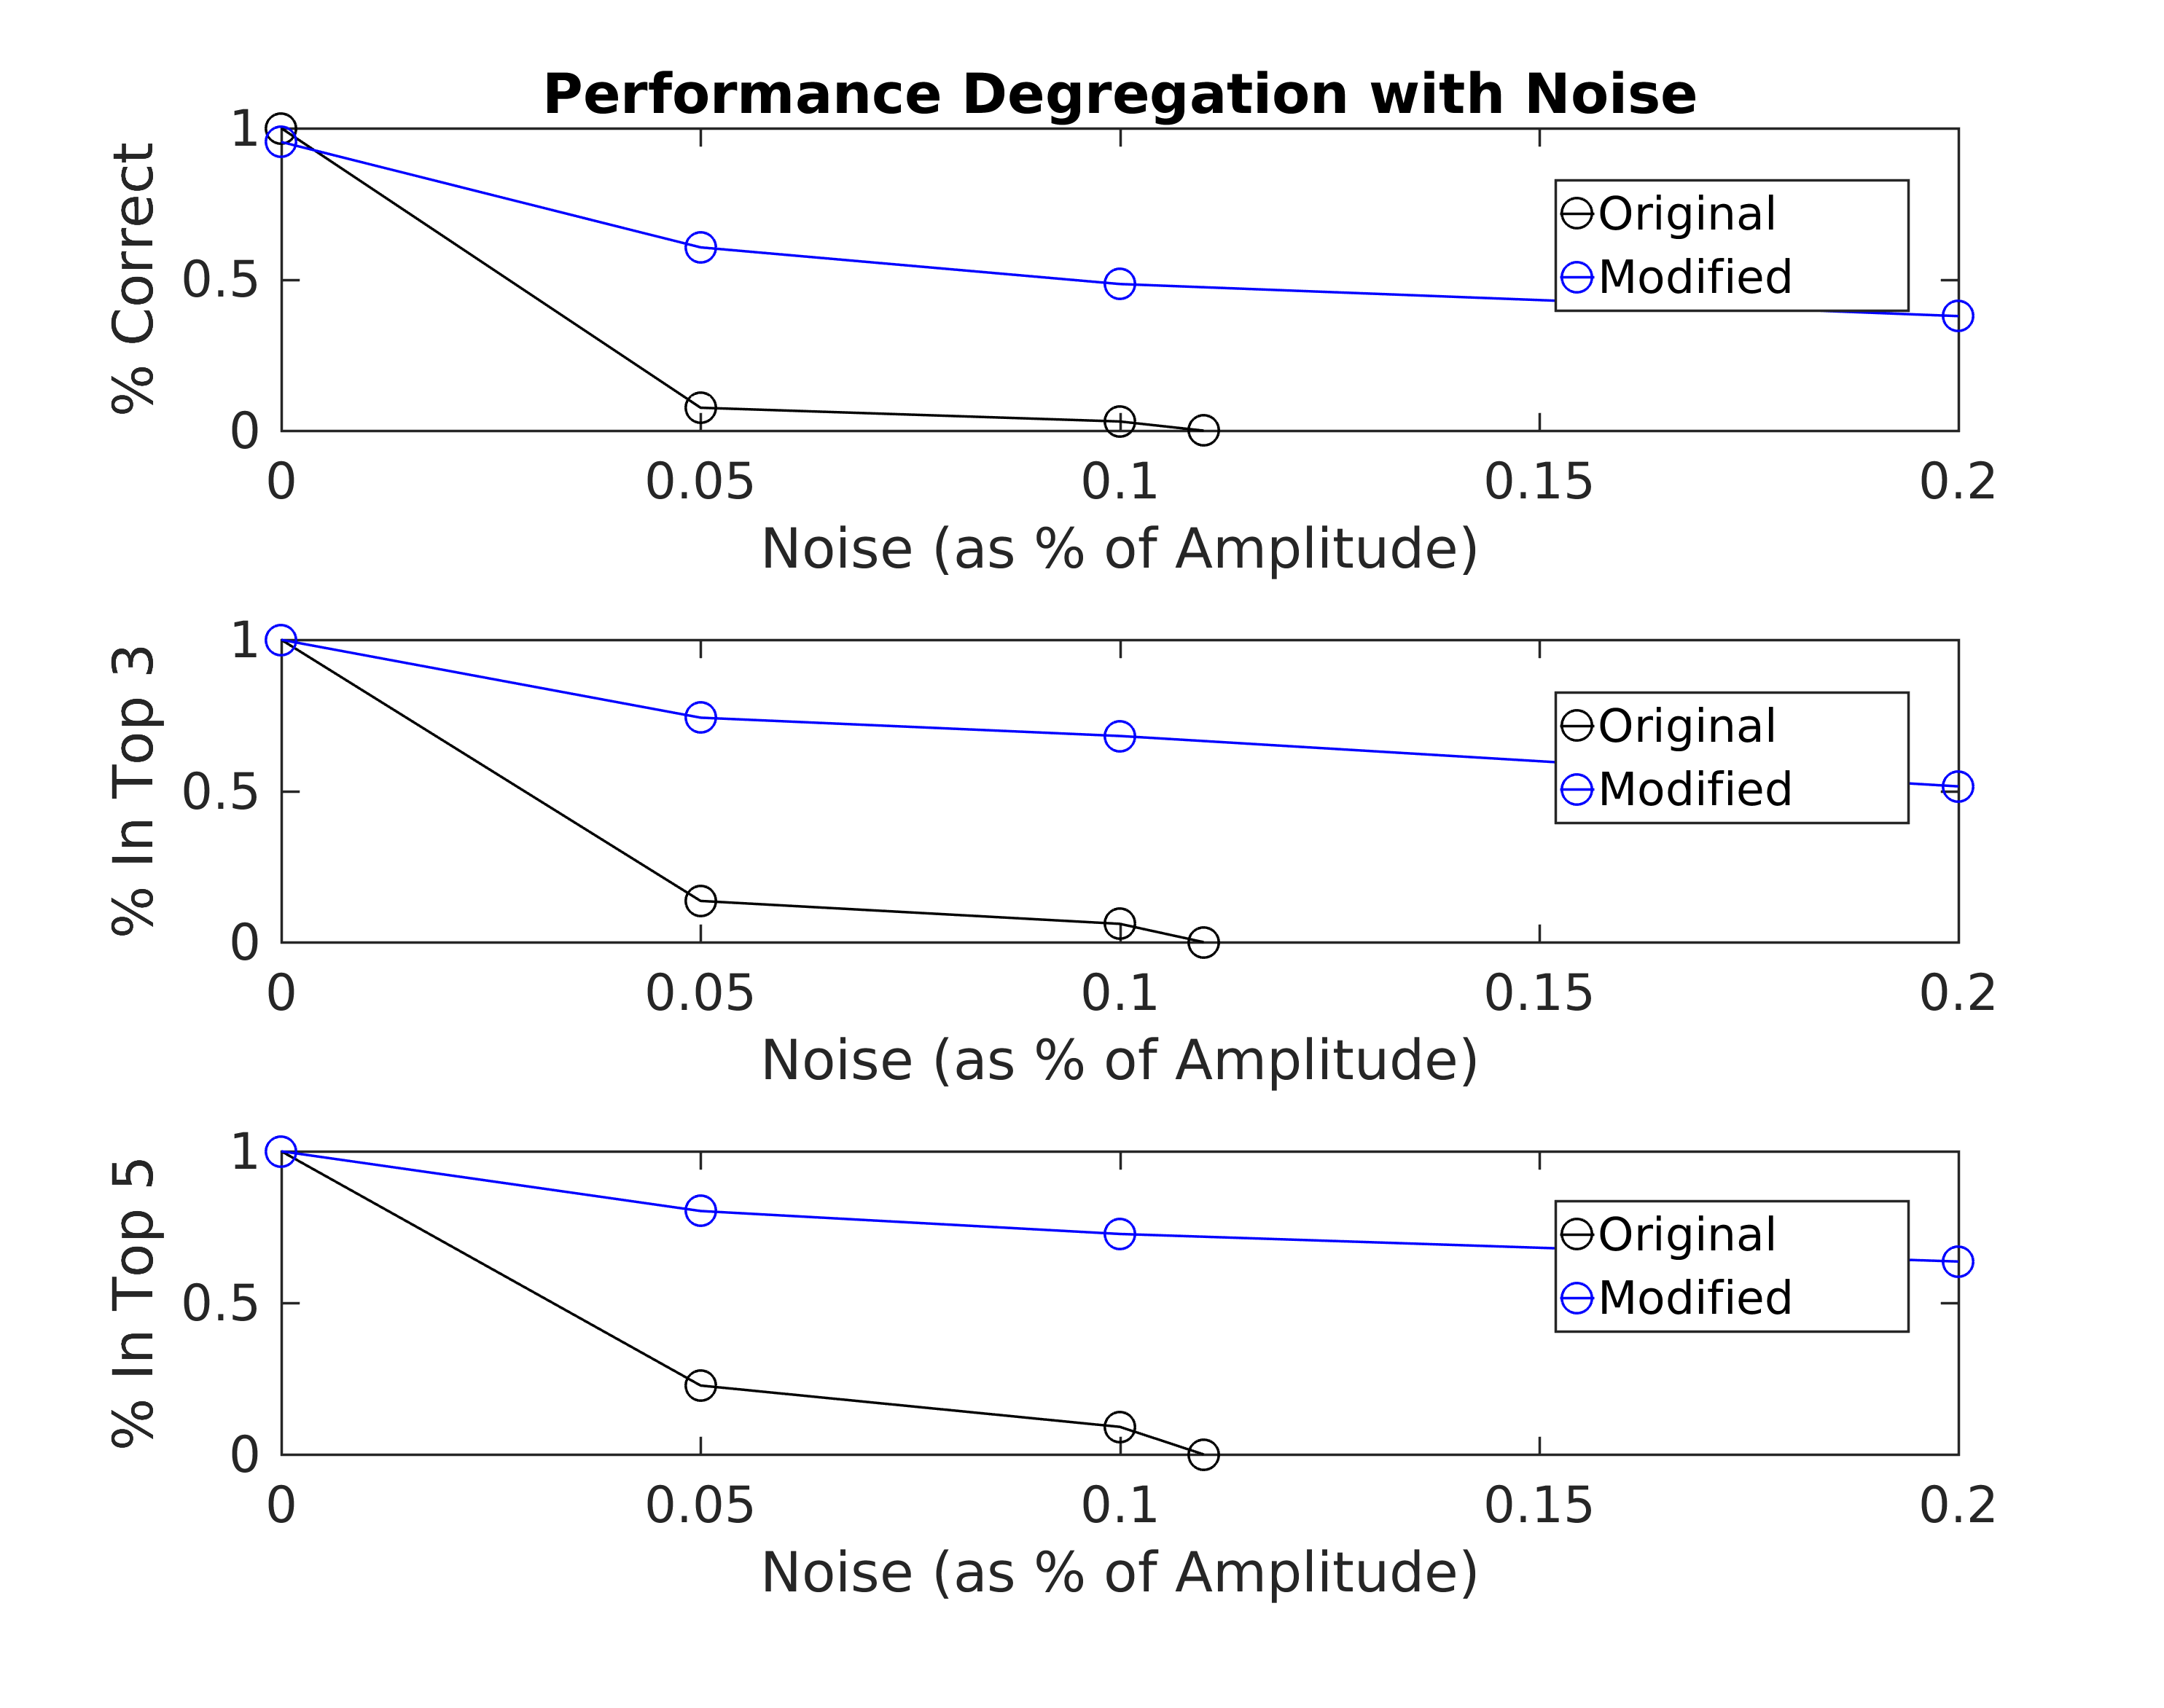
\includegraphics[width=13cm]{Comparison2.png}
\caption{Results when applied to Power Systems case with three sensors placed on the 57 bus system. The three plots compare the effects of noise on $L$ and $M$, plotted in blue and black respectively. Noise (on the x axis) is added as a percentage of maximum amplitude. Performance in the non-noisy case is comparable for $L$ and $M$, although $L$ performs slightly worse due to ``misidentifications'' of sequential lines. }
\end{figure}

\end{document}